\section{Condizioni}\index{Condizioni}

\begin{enfasi}
La grandezza dell'uomo è nella decisione di essere più forte della sua condizione. (Albert Camus)
\end{enfasi}

%{\small
\begin{multicols}{2}

\label{condizioni}

\textbf{Accelerato}\index{Accelerato}\hypertarget{Accelerato}{}\label{Accelerato}: una creatura Accelerata ottiene un numero di Azioni bonus per round pari al valore di Accelerato. La durata è indicata dopo la \emph{"\"}. Quando è indicata la durata si intente fino alla fine del round di scadenza. Es. Accelerato 1/3r, Accelerato 2/-.

\textbf{Aumento Categoria di danno}\index{Aumento Dadi}\index{Taglia dei dadi}: quando la regola vi dice di aumentare la taglia o categoria di un dado seguite questo schema.

1d4 -> 1d6 -> 1d8 -> 1d10 (1d12)-> 2d6 -> 2d8 -> 2d10 -> 3d6 -> 3d8 -> 3d10.

\textbf{Accecato}:\index{Accecato} Il personaggio non riesce a vedere nulla. subisce penalità -2 alla maggior parte delle Competenze basate su Forza e Destrezza.

Tutte le prove o le attività basate sulla visione (come ad esempio leggere, o eventuali prove di Consapevolezza basate sulla vista) falliscono automaticamente. Tutti gli avversari vengono considerati dotati di invisibilità nei confronti del personaggio accecato.

I personaggi accecati considerano il terreno sempre come difficile e devono effettuare una prova di Acrobatica con DC 12 per muoversi più veloci della propria velocità dimezzata. Le creature che falliscono questa prova cadono a terra Prone. I personaggi che rimangono per lungo tempo accecati possono abituarsi ad alcune di queste penalità e iniziare a superarne alcune, a discrezione del Narratore.

Chi attacca una creatura per lei invisibile ha un -1d6 al Tiro per Colpire, la creatura invisibile che attacca una creatura che non la vede ha +1d6 al Tiro per Colpire

\textbf{Affascinato}:\index{Affascinato} Una creatura affascinata non può attaccare o bersagliare chi l'ha affascinata con attacchi, capacità speciali o effetti magici dannosi.

Qualsiasi potenziale minaccia causata da chi l'ha affascinata, come ad esempio una creatura ostile in avvicinamento, consente alla creatura affascinata un nuovo Tiro Salvezza contro l'effetto del fascino. Qualsiasi minaccia palese, come ad esempio qualcuno che estrae un'arma, lancia un incantesimo o punta un'arma a distanza verso la creatura affascinata, interrompe automaticamente l'effetto.

Un alleato della creatura affascinata può scuoterla per permettergli un nuovo Tiro Salvezza spendendo 2 Azioni.

L'affascinatore ha +1d6 su qualsiasi prova di Competenza per interagire socialmente con la creatura.

L'effetto di Affascinato termina se la creatura diventa morente.

\textbf{Affaticato}\index{Affaticato}\hypertarget{affaticato}{}\index{Esausto}\label{affaticato}: Un personaggio affaticato non può correre o Caricare e subisce una penalità -1 a Difesa e Prove (Tiro per Colpire, Competenze, Magia, Tiri Salvezza) e Movimento. Se compie qualsiasi cosa normalmente affaticante aumenta il suo grado di Affaticato e prende penalità anche al movimento ed alle prove di competenza di Base.

Se un personaggio non dorme almeno 8 ore (TS Tempra DC 17) nell'arco di 24 ore o dorme con un armatura media o pesante alla mattina è affaticato.

Dopo 1 ora di completo riposo (o \hyperlink{Ristorare Inferiore}{Ristorare Inferiore}), un personaggio Affaticato 2 diventa Affaticato.

\medskip

\textbf{Tabella: Livelli Affaticamento}\index[Tabelle]{Tabella Livelli Affaticamento}

\medskip

\noindent\begin{tabularx}{\linewidth}{Xcc}
	\toprule
\rowcolor{gray!20}\textbf{Condizioni}& \textbf{Penalità}&\textbf{Recupero}\\
\toprule
Affaticato 		&	1 		&	1h\\
\rowcolor{gray!20}Affaticato 2	&	2		&	1h\\
Affaticato 3	&	3		&	8h\\
\rowcolor{gray!20}Affaticato 4	&	4		&	12h\\
Affaticato 5	&	Svenuto	&	6h\\
\rowcolor{gray!20}Affaticato 6	&	Morte	&	--
\end{tabularx}

%\begin{tabularx}{\linewidth}{|c|X|l|}
%
%\textbf{Liv.} & \textbf{Effetto} & \textbf{Rec.}\\
%
%1 & -1d6 alle Prove di Competenza&1h\\
%2 & Velocità di movimento dimezzata &1h\\
%3 & -1d6 ai Tiri per Colpire e Tiri Salvezza &8h\\
%4 & Punti ferita massimi dimezzati &12h\\
%5 & Svenuto &6h\\
%6 & Morte &-\\
%
%\end{tabularx}

\medskip

Dopo 8 ore di riposo una creatura passa da Affaticato 3 ad Affaticato 2 e dopo un'altra ora passa ad Affaticato, purché non subisca ulteriori affaticamenti.

\medskip

\textbf{Afferrato}\index{Afferrato}: Una creatura afferrata non può muoversi ma può provare a Spingere. Deve usare due Azioni per liberarsi, vedi sezione combattimento \hyperlink{afferrareunavversario}{Afferrare un avversario}.

Può attaccare con armi in mischia se piccole o a mani nude. Ha -2 alla Difesa ed è Distratto.

La condizione vale su chi è afferrato e su chi afferra.

\textbf{Amichevole}:\index{Amichevole} Una creatura amichevole non attaccherà il personaggio se non minacciata esplicitamente.

\textbf{Annegare/Trattenere il fiato}: \index{Annegare}\index{Trattenere il fiato}\index{Soffocare} Qualsiasi personaggio può trattenere il fiato per un numero di round pari 6 round per il suo punteggio di Costituzione, con un minimo di 3 round. Per ogni Azione compiuta la durata restante diminuisce di 1 round. Trascorso questo periodo di tempo, il personaggio deve effettuare un Tiro Salvezza su Tempra con DC 12 ogni round per continuare a trattenere il fiato. Ogni round, la DC aumenta di 2. Vedi pag. \pageref{trattenereilfiato}

\textbf{Assordato}:\index{Assordato}\index{Sordo} Un personaggio assordato non può ascoltare. Fallisce automaticamente tutte le prove di Consapevolezza basate sul suono e si considera Distratto nel lancio degli incantesimi con componenti almeno verbali.

I personaggi che rimangono assordati per lunghi periodi di tempo, possono abituarsi a queste penalità e superarne alcune, a discrezione del Narratore.

\textbf{Avvelenato}\index{Avvelenato}: si considera avvelenato qualsiasi soggetto sotto l'influenza di un veleno o pozione, indipendentemente che questa stia già producendo gli effetti o li debba ancora produrre dato il tempo dell'insorgenza. Una creatura immune al danno da Veleno non può avere la condizione Avvelenato.

\textbf{Bloccato}\index{Bloccato}\hypertarget{bloccato}{}: una creatura bloccata ha entrambe le braccia bloccate. Può spostarsi provando a Spingere, deve usare due Azioni per liberarsi (vedi \hyperlink{afferrareunavversario}{Afferrare un avversario}). Prende -4 alla Difesa ed ai Tiri Salvezza su Riflessi.

Un incantatore Bloccato è Distratto e deve effettuare una Prova di Magia con Successo Critico Magico o non riesce a formulare magie. -1d6 al Tiro per Colpire.

Chi ha Bloccato una creatura si considera Afferrato.

\textbf{Colpo di Grazia}:\index{Colpo di Grazia} Come unica Azione nel round, una creatura può utilizzare un'arma da mischia per infliggere un colpo di grazia ad un personaggio inabile o indifeso. Può anche usare un arco o una balestra, l'importante è che sia adiacente al bersaglio.

L'attaccante colpisce automaticamente ed infligge tre colpi critici. Le creature immuni ai colpi critici non possono subire un Colpo di Grazia.

\textbf{Confuso}: \index{Confuso}\index{Confusione}\hypertarget{confusionecondizione}{}Una creatura confusa è mentalmente ottenebrata e non può agire normalmente. Una creatura confusa non riesce a distinguere un alleato da un nemico e considera tutti come nemici.

Se una creatura confusa è attaccata, attacca sempre l'ultima creatura che la ha attaccata, finché quella creatura non muore o esce dalla sua visuale.

Tirate un dado sulla tabella seguente all'inizio di ogni round della creatura confusa per vedere quello fa in quel round.

\medskip

\noindent\begin{tabularx}{\linewidth}{lX}
	\toprule
\rowcolor{gray!20}\textbf{d10} & \textbf{Comportamento} \\
\toprule
1 & La creatura usa tutte le sue Azioni per per muoversi in una direzione casuale. Per determinare la direzione tira un d8\\
\rowcolor{gray!20}2-5 & La creatura non fa nulla per tutto il round\\
6 &  La creatura effettua un attacco contro se stessa e finisce il round\\
\rowcolor{gray!20}7-8 & La creatura effettua un attacco contro una creatura determinata a caso entro 1 Azione di Movimento. Se è stata colpita il round precedente attaccherà la creatura che l'ha colpito. Fatto l'attacco il round termina.\\
9-10 & La creatura può agire e muoversi normalmente.
\end{tabularx}

\medskip

Una creatura confusa che non è in grado di eseguire l'azione indicata non farà altro che balbettare in modo incoerente. Gli aggressori non hanno alcun vantaggio speciale quando attaccano una creatura confusa. Qualsiasi creatura confusa che venga attaccata, attacca automaticamente a sua volta il suo aggressore.

\textbf{Distratto}\index{Distratto}: Se l'incantatore è severamente distratto, impedito, disturbato, sanguinante, afferrato, cerca di nascondere il lancio della magia, è sotto attacco mentre cerca di lanciare un incantesimo deve effettuare una Prova di Magia.

\textbf{Dominato}:\index{Dominato} Se si ha un linguaggio in comune, si può generalmente costringere il soggetto ad eseguire i comandi entro i limiti delle sue capacità. Se non si condivide nessun linguaggio, si possono impartire solo comandi di base come \emph{vieni qui}, \emph{vai lì}, \emph{combatti} o \emph{stai fermo}. Si è a conoscenza di ciò che il soggetto sta provando ma non si ricevono percezioni sensoriali dirette da lui, né si può comunicare con lui telepaticamente.

Una volta impartito un ordine alla creatura dominata, questa continua a tentare di eseguirlo con l'esclusione di tutte le altre attività ad eccezione di quelle necessarie per la sopravvivenza quotidiana (come mangiare, dormire e così via). Grazie a questo limitato spettro di attività, una prova di Consapevolezza con DC 15 (invece che DC 25) può determinare se il comportamento del soggetto è stato influenzato da un effetto di ammaliamento.

Concentrandosi completamente sull'incantesimo (2 Azioni), si possono ricevere percezioni sensoriali come vengono interpretate dalla mente del soggetto, anche se questo non può comunque comunicarle. Non si può in realtà vedere attraverso gli occhi del soggetto, quindi non è come se si fosse presenti, ma ci si può rendere conto di cosa sta succedendo.

Ovviamente ordini palesemente autodistruttivi non vengono eseguiti. Una volta stabilito il controllo, il raggio di azione entro il quale può essere mantenuto è illimitato purché entrambi i soggetti rimangano sullo stesso piano. Non c'è bisogno di vedere il soggetto per controllarlo. Se ogni giorno non si trascorre almeno 1 minuto a concentrarsi sull'incantesimo, il soggetto riceve un nuovo Tiro Salvezza per liberarsi dal controllo.

\textbf{Dormire}\index{Dormire}: Ogni volta che un personaggio termina un periodo di 24 ore senza dormire almeno 8 ore, deve superare un Tiro Salvezza su Tempra con DC 17, altrimenti diventa Affaticato. Ogni riposo mancato ulteriore lo renderà ancora più Affaticato cumulando le penalità relative.
Se il personaggio resta sveglio per più giorni, lottare contro il sonno diventa più difficile. Dopo le prime 24 ore, la DC aumenta di 4 per ogni periodo consecutivo di 24 ore trascorso senza aver dormito 8 ore. La DC torna a 17 quando il personaggio completa un riposo di almeno 8 ore.

\textbf{Fiancheggiare}\index{Fiancheggiare}\index{Fiancheggiato}: una creatura è fiancheggiata se ha due avversari non affiancatati attorno a se ed una ipotetica linea che unisce gli avversari attraversa il quadretto della creatura completamente. Le due creature prendono +2 al Tiro per Colpire o alla Difesa.

\textbf{Impreparato / Sorpreso}\index{Impreparato}\index{Surpreso}\label{impreparato}:
Una creatura sorpresa / impreparata ha una penalità di -2 a Difesa ed ai Tiri Salvezza su Riflessi. Non potrà reagire, non userà Azioni o Reazioni se non esplicitamente permesse; dal round successivo potrà dichiarare l'iniziativa ed agire normalmente.

\textbf{Inabile}\index{Inabile}: Una creatura inabile non può effettuare azioni o reazioni. È Impreparata (-4 a Difesa ed ai Tiri Salvezza su Riflessi)

\textbf{In Lotta}:\index{Lotta} Una creatura in lotta è trattenuta da una creatura, da una trappola o da un effetto. Vedi \textbf{Afferrato}.

\textbf{Indifeso}:\index{Indifeso}\index{Addormentato}\index{Privo di sensi}\index{Morente}\hypertarget{indifeso}{}\hypertarget{morente}{}\label{morente} Un personaggio addormentato, Privo di Sensi, Morente o per qualche altro motivo completamente alla mercé dei suoi avversari, è considerato Indifeso.

Una creatura Indifesa non può compiere Azioni o Reazioni ne parlare, gli attacchi in mischia contro di lei hanno +1d6 di bonus. Non è consapevole di ciò che gli accade intorno. La creatura lascia cadere qualsiasi cosa impugni e cade prona.

La creatura fallisce automaticamente i Tiri Salvezza su Tempra e Riflessi.

La creatura perde il bonus di Destrezza alla Difesa.

\textbf{Intralciato}:\index{Intralciato}\hypertarget{intralciato}{}\label{intralciato} Un personaggio intralciato ha difficoltà di movimento, ma può comunque provare a muoversi, a meno che i legami che lo intralciano non siano ancorati a un oggetto immobile o impugnati da una forza contrapposta.

Una creatura intralciata tratta il terreno come Difficile, non può Correre o Caricare, subisce penalità -2 alla Difesa ed ai Tiri per Colpire.

Un personaggio intralciato che cerca di lanciare un incantesimo si considera Distratto.

\textbf{Invisibile}:\index{Invisibile} Le creature invisibili non sono percepibili dalla vista.
Chi attacca una creatura per lei invisibile ha un -1d6 al Tiro per Colpire, la creatura invisibile che attacca una creatura che non la vede ha +1d6 al Tiro per Colpire.

\textbf{Morente} \index{Morente}: Un personaggio morente ha -1 Punti Ferita. È indifeso. Ogni round perde 1 punto ferita finché muore o viene curato. Vedi \textbf{Indifeso}

\textbf{Nauseato}\index{Nauseato}: Se la penalità non è già espressa una creatura nauseata ha -1d6 ai Tiri per Colpire, Tiri Salvezza e Prove Competenze.

\textbf{Morto}:\index{Morto}\hypertarget{morto}{} L'anima del personaggio abbandona permanentemente il suo corpo. I personaggi morti non possono beneficiare delle cure normali o magiche, e non possono essere riportati in vita da un incantesimo. Solo un Patrono ha sufficiente potere per riportare l'anima nel corpo e riportare in vita la creatura. La Scuola di Necromanzia ha incantesimi per rianimare un corpo come non morto.

\textbf{Paralizzato}: \index{Paralizzato} Un personaggio paralizzato non può compiere Azioni o Reazioni ne parlare, gli attacchi in mischia contro di lei hanno +1d6 di bonus e perde il bonus alla Difesa dato dalla Destrezza. La creatura è consapevole di ciò che ha intorno, non lascia cadere gli oggetti. La creatura fallisce automaticamente i Tiri Salvezza su Riflessi.

Una creatura alata in volo, nel momento in cui viene paralizzata non può più battere le ali e precipita. Un nuotatore paralizzato non può più Nuotare e potrebbe annegare.

Il terreno occupato da una creatura paralizzata (o morta) si considera come terreno difficile.

\textbf{Perdita di punti Caratteristica}\index{Perdita di punti Caratteristica}\index{Caratteristica perdita punti}: quando si i punteggi Caratteristica diminuiscono ricordarsi di togliere eventuali Punti Ferita 1 per punto di Costituzione perso per livello, abbassare Tiri Salvezza (Destrezza, Costituzione, Saggezza), Tiri per Colpire (Forza e Destrezza), \textbf{Difesa:} (Difesa). Se non indicato come permanente si recupera 1 punto in tutto di Caratteristica al giorno di riposo.

\textbf{Pietrificato}: \index{Pietrificato}Un personaggio pietrificato è stato trasformato in pietra ed è privo di sensi ed \textbf{Indifeso}, viene considerato un oggetto.

Se un personaggio pietrificato si incrina o si rompe, ma i pezzi rotti sono uniti al corpo quando ritorna di carne, il personaggio non viene ferito o danneggiato. Se il corpo pietrificato del personaggio è incompleto quando viene ritrasformato in carne, il corpo rimane incompleto e potrebbe avere una qualche perdita permanente di Punti Ferita e/o altre menomazioni.

La creatura dispone di resistenza a tutti i danni. La creatura è immune ai veleni e le malattie, ma gli eventuali i veleni e le malattie già presenti nel suo sistema vengono solo sospesi, non neutralizzati. La creatura non ha percezione dell'ambiente ne capacità cognitive.

\textbf{Paura, Spaventato}:\index{Paura}\index{Spaventato}\hypertarget{condizionepaura}{}
Una creatura spaventata ha -1d6 ai Tiri per Colpire, Tiri Salvezza e Prove Competenza finché la sorgente della sua paura è visibile. Una creatura spaventata non può avvicinarsi volontariamente alla sorgente della sua paura.

\textbf{Privo di sensi}\index{Privo di sensi}: si considera che sia \textbf{Indifeso}.

\textbf{Prono}\index{Prono}: chi è prono ha un -4 ad attaccare ed un -4 alla Difesa. Alzarsi da prono costa 1 Azione. Non si può diventare proni se si vola.

Il giocatore può eseguire una prova di Acrobatica se fa 13 o più costa 1 Azione immediata. Se fai un Fallimento Critico nella prova non puoi fare altre azioni quel round e rimani prono.

Quando sei prono puoi strisciare\index{Strisciare}\index{Carponi} o muoverti a carponi. Il terreno si considera difficile e sei comunque considerato ancora prono finché non ti alzi.

\textbf{Punti Ferita Massimi}\index{Punti Ferita massimi}: una creatura che subisca un attacco che abbassa i Punti Ferita Massimi deve calare prima i Punti Ferita Massimi attuali e poi diminuisce dello stesso ammontare i Punti Ferita attuali se non già tolti. Se i Punti Ferita Massimi arrivano a 0 la creatura è morta. I Punti Ferita massimi si recuperano nella misura di 1 per valore di Costituzione per 8 ore di riposo.

\textbf{Resistenza al Danno}\index{Resistenza al Danno}: una creatura che abbia Resistenza al Danno si considera che dimezzi automaticamente il danno dalla fonte specificata, es. Resistenza al Danno: Suono. La Resistenza al Danno può essere indicata anche con un valore numerico, es. Resistenza al Danno: Fuoco 10. In questo caso la protezione funziona sui primi 10 danni subiti, in caso di effetto che concede un Tiro Salvezza per dimezzare, prima si toglie l'ammontare della protezione al totale, poi si esegue il Tiro Salvezza per dimezzare il danno residuo.

\textbf{Stordito/Svenuto}:\index{Stordito}\index{Svenuto} si considera che sia \textbf{Indifeso}. Può parlare a fatica.

\textbf{Trattenere il fiato}: leggi \textbf{Annegare/Trattenere il fiato}

\textbf{Rallentato}\index{Rallentato}: una creatura rallentata non è in grado di eseguire tutte le sue possibili Azioni nel round. Rallentato viene sempre indicato con due valori, il primo indica quante Azioni in meno si fanno a round, il secondo la durata dell'effetto, se segnato con un - allora non ha una fine indicata. Quando è indicata la durata si intente fino alla fine del round di scadenza. Es. Rallentato 1/3r, Rallentato 2/-.

\textbf{Ristretto}\index{Ristretto}\hypertarget{ristretto}{} : due creature medie o piccole che condividono lo stesso quadretto di mappa si considerano ristretti. Entrambe le creature prendono -1d6 al Tiro per Colpire ed alla Difesa (-4) finché condividono lo spazio. Una creature può condividere il quadretto con una creatura di taglia almeno tre volte più grande senza penalità.

\textbf{Rotto}\index{Rotto}: La condizione rotto ha i seguenti effetti, a seconda dell'oggetto:

- Se l'oggetto è un'arma, tutti gli attacchi effettuati con l'oggetto subiscono penalità -2 al Tiro per Colpire ed ai danni. Tali armi ottengono un Colpo Critico soltanto con un 3 volte 6 ed infliggono al massimo solo 1 volta il danno in aggiunta.

- Se l'oggetto è un'armatura o uno scudo, il bonus che concede alla Difesa è dimezzato, arrotondando per eccesso. L'armatura rotta raddoppia la penalità di armatura alla Prova sulle Competenze.

- Se l'oggetto è un attrezzo necessario per una Competenza, tutte le prove di Competenza di Base effettuate con esso subiscono penalità -2.

- Se l'oggetto è una Bacchetta o un Bastone, utilizzate il doppio delle cariche necessarie ogni volta che viene usato.

- Se l'oggetto non rientra in nessuna delle precedenti categorie, la condizione rotto non ha effetto sul suo uso. Gli oggetti con condizione rotto, a prescindere dal tipo, valgono il 25\% del loro costo normale. Se l'oggetto è magico, può essere riparato soltanto con l'incantesimo \hyperlink{Fabbricare}{Fabbricare} utilizzata da un incantatore di livello uguale o superiore a quello che ha creato dell'oggetto.

\textbf{Sanguinante}\index{Sanguinamento}\hypertarget{sanguinamento}{}: Una creatura che sta subendo danni da sanguinamento subisce la quantità di danno indicata all'inizio del suo round. La Riduzione del danno (DR) non funziona sul danno da sanguinamento. Il sanguinamento può essere ridotto di un punto superando una prova di Pronto Soccorso con DC 12, 2 Azioni.
Per ogni valore di Sanguinamento sopra 1 la difficoltà aumenta di 2.

Un trattamento di 1 minuto garantisce 1 successo, senza prova. Ogni Successo Critico riduce il sanguinamento di un punto ulteriore. Alcuni effetti di sanguinamento causano un danno di caratteristica o persino un risucchio di caratteristica.

Il sanguinamento si riduce di 1 per ogni dado di cura della Pozione o Incantesimi. Se i Punti Ferita del soggetto vengono riportati al valore massimo il sanguinamento termina. Il sanguinamento prosegue anche se la creatura è \hyperlink{morente}{morente}.\index{Sanguinamento e cure}

Se non indicato diversamente il danno da sanguinamento si cumula fino ad un massimo di 10 Punti Ferita a round. Il danno da sanguinamento viene indicato con Sanguinamento valore/valore massimo, dove valore è il punteggio di sanguinamento causato dall'attacco e valore massimo è il punteggio di sanguinamento massimo che si può raggiungere.

Se la creatura diventa morente, va a Punti Feriti negativi, e poi viene riportata in vita perde gli effetti del Sanguinamento.

\textbf{Vulnerabilità}\index{Vulnerabilità}: funziona al contrario della Resistenza. Il danno viene raddoppiato prima dell'eventuale Tiro Salvezza.

\end{multicols}

\vfill

\begin{enfasi}
	Facilis descensus Averno (Facile è la discesa agli inferi). Eneide, Virgilio
\end{enfasi}

\pagebreak

\noindent\rule{\textwidth}{0.4pt}

\subsection{Tabelle per tiri casuali}

{\small \setlength{\parindent}{0cm}{

\begin{multicols}{2}

\textbf{Tabella Fonti di Energia}\index{Tabella Casuale - Fonti di Energia}\label{fontienergia}\hypertarget{fontienergia}{}

\noindent\begin{tabularx}{\linewidth}{ll|ll}
	\toprule
\rowcolor{gray!20}3d6 &Energia&&\\
3-5&Energia Neg.& 6-8&Energia Pos.\\
\rowcolor{gray!20}9-11&Fuoco & 12-13&Freddo\\
14&Elettricità & 15&Suono\\
\rowcolor{gray!20}16&Luce & 17&Vuoto\\
18&Forza&&\\
\end{tabularx}

\medskip

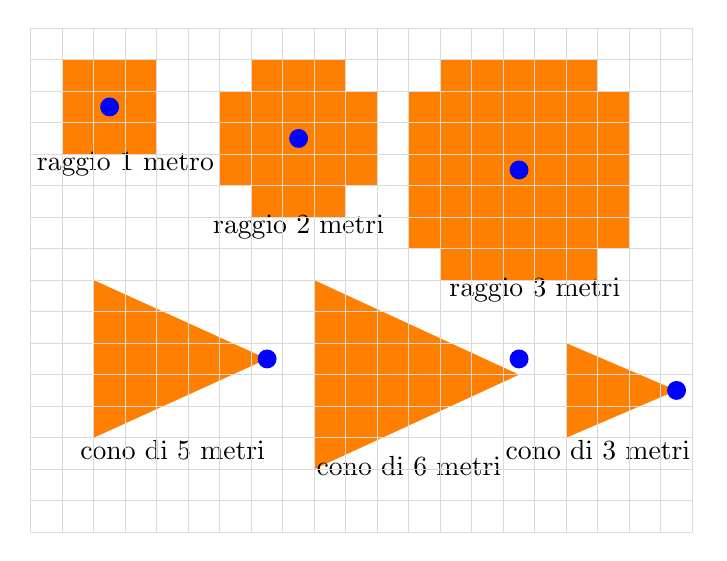
\begin{tikzpicture}[scale=0.4]

	\fill[orange] (1,17) rectangle (4,20);
	\fill[blue] (2.5,18.5) circle (0.3);
	\node at (3,16) [above] {raggio 1 metro};

	\fill[orange] (6,15) rectangle (11,20);
	\fill[white] (5,20) rectangle (6,21);
	\fill[white] (6,19) rectangle (7,20);
	\fill[white] (10,15) rectangle (11,16);
	\fill[white] (6,15) rectangle (7,16);
	\fill[white] (10,19) rectangle (11,20);
	\fill[blue] (8.5,17.5) circle (0.3);
	\node at (8.5,14) [above] {raggio 2 metri};

	\fill[orange] (12,13) rectangle (19,20);
	\fill[white] (12,19) rectangle (13,20);
	\fill[white] (18,13) rectangle (19,14);
	\fill[white] (12,13) rectangle (13,14);
	\fill[white] (18,19) rectangle (19,20);
	\fill[blue] (15.5,16.5) circle (0.3);
	\node at (16,12) [above] {raggio 3 metri};

	\fill[orange] (2,8) -- (7.5,10.5) -- (2,13) -- cycle;
	\fill[blue] (7.5,10.5) circle (0.3);
	\node at (4.5,7) [above] {cono di 5 metri};

	\fill[orange] (17,8) -- (20.5,9.5) -- (17,11) -- cycle;
	\fill[blue] (20.5,9.5) circle (0.3);
	\node at (18,7) [above] {cono di 3 metri};

	%\fill[orange] (9,7) -- (15.5,10.5) -- (9,13) -- cycle;
	%\fill[blue] (15.5,10.5) circle (0.3);
	%\node at (12,6.5) [above] {cono di 6 metri};

	\fill[orange] (9,7) -- (15.5,10) -- (9,13) -- cycle;
	\fill[blue] (15.5,10.5) circle (0.3); % Punto blu sulla punta destra
	\node at (12,6.5) [above] {cono di 6 metri};

	% Cubo di 3 quadretti di lato
	%\fill[orange] (2,2) -- (5,2) -- (5,5) -- (2,5) -- cycle; % Faccia frontale
	%\fill[orange] (5,2) -- (6,3) -- (6,6) -- (5,5) -- cycle; % Faccia destra
	%\fill[orange] (2,5) -- (5,5) -- (6,6) -- (3,6) -- cycle; % Faccia superiore

	% Cubo di 6 quadretti di lato
	%\fill[orange] (8,2) -- (14,2) -- (14,8) -- (8,8) -- cycle; % Faccia frontale
	%\fill[orange] (14,2) -- (16,4) -- (16,10) -- (14,8) -- cycle; % Faccia destra
	%\fill[orange] (8,8) -- (14,8) -- (16,10) -- (10,10) -- cycle; % Faccia superiore

	% Draw the base grid (20x15)
	\foreach \x in {0,...,20}
	\foreach \y in {5,...,20}
	\draw[gray!30] (\x,\y) grid (\x+1,\y+1);

\end{tikzpicture}

\medskip

Il punto blu determina l'origine dell'incantesimo

\bigskip

\textbf{Esempi portata dei nemici}

\medskip

\textbf{Tabella: forme degli incantesimi - Sfera e Cono}\index[Tabelle]{Tabella forme degli incantesimi - Sfera e Cono}

\medskip


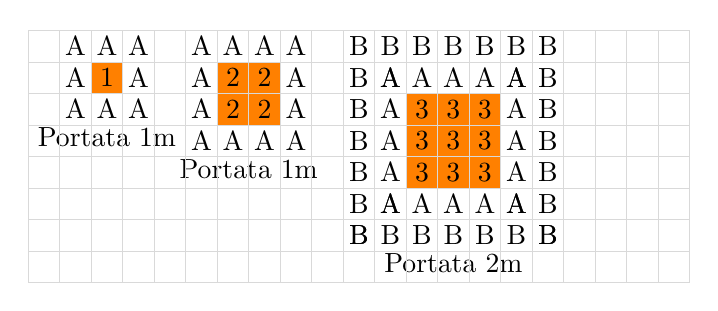
\begin{tikzpicture}[scale=0.4]

	\fill[orange] (1,18) rectangle (2,19);
	\node at (1.5,18.5) {1};

	\foreach \x in {-1,...,1} {
		\node at (\x+1.5,17.5) {A};
		\node at (\x+1.5,19.5) {A};
	}

	\foreach \y in {18} { \node at (+0.5,\y+0.5) {A};
		\node at (2.5,\y+0.5) {A}; }

	\node at (1.5,16) [above] {Portata 1m};

	% Quadrato centrale 2x2 con il numero 2 dentro
	\fill[orange] (5,17) rectangle (7,19);
	\node at (5.5,17.5) {2};
	\node at (5.5,18.5) {2};
	\node at (6.5,17.5) {2};
	\node at (6.5,18.5) {2};

	% Lettere A intorno al quadrato centrale 2x2
	\foreach \x in {3,...,6} {
		\node at (\x+1.5,19.5) {A}; % Sopra
		\node at (\x+1.5,16.5) {A}; % Sotto
	}
	\foreach \y in {9,...,10} {
		\node at (4.5,\y+8.5) {A}; % Sinistra
		\node at (7.5,\y+8.5) {A}; % Destra
	}

	\node at (6,15) [above] {Portata 1m};

	% Quadrato 3x3 con il numero 3 dentro, spostato a sinistra di 1 quadretto e alzato di 1 quadretto
	\fill[orange] (11,15) rectangle (14,18);
	\node at (11.5,17.5) {3};
	\node at (12.5,17.5) {3};
	\node at (13.5,17.5) {3};

	\node at (11.5,16.5) {3};
	\node at (12.5,16.5) {3};
	\node at (13.5,16.5) {3};

	\node at (11.5,15.5) {3};
	\node at (12.5,15.5) {3};
	\node at (13.5,15.5) {3};

	% Prima cornice di quadretti con la lettera A
	% Sopra e sotto il quadrato 3x3
	\foreach \x in {10,...,14} {
		\node at (\x+0.5,14.5) {A};
		\node at (\x+0.5,18.5) {A};
	}

	% Ai lati del quadrato 3x3
	\foreach \y in {13,...,17} {
		\node at (10.5,\y+1.5) {A};
		\node at (14.5,\y+1.5) {A};
	}

	% Seconda cornice di quadretti con la lettera B
	% Sopra e sotto la prima cornice
	\foreach \x in {9,...,15} {
		\node at (\x+0.5,19.5) {B};
		\node at (\x+0.5,13.5) {B};
	}

	% Ai lati della prima cornice
	\foreach \y in {13,...,18} {
		\node at (9.5,\y+0.5) {B};
		\node at (15.5,\y+0.5) {B};
	}
	\node at (12.5,12) [above] {Portata 2m};

	\foreach \x in {-1,...,19}
	\foreach \y in {12,...,19}
	\draw[gray!30] (\x,\y) grid (\x+1,\y+1);

\end{tikzpicture}

\textbf{Generatori Effetti Fallimento Critico in Attacco}\index{Tabella Casuale - Fallimento critico con armi}\label{tabellafallimentiarmi}\hypertarget{tabellafallimentiarmi}{}

\noindent\begin{tabularx}{\linewidth}{l|X}
	\toprule
\rowcolor{gray!20}\textbf{3d6} & \textbf{Effetto}\\
\toprule
3& Sei imbarazzato del tuo colpo, ma non succede nulla di particolare\\
\rowcolor{gray!20}4& Ti sbilanci. Fino a all'inizio del prossimo round hai -2 alla Difesa\\
5& Metti male il piede. Fino alla fine del prossimo round tratti il terreno come difficile\\
\rowcolor{gray!20}6& Perdi il fiato. Fino all'inizio del prossimo round ha -1 Forza\\
7& Piroetta. Ti sposti in una direzione casuale di 1 metro\\
\rowcolor{gray!20}8& Goffo. Fino a all'inizio del prossimo round hai -4 alla Difesa\\
9& Occhio pesto. Fino alla fine del round prossimo ogni avversario gode di copertura leggera\\
\rowcolor{gray!20}10 & Mani di burro. Ti cade l'arma\\
11 & Strappo muscolare. Il prossimo attacco non aggiunge la Forza al danno\\
\rowcolor{gray!20}12 & Caviglia fragile. Portando il colpo inciampi. Cadi prono\\
13 & Ti cade l'arma a 3 metri in una direzione casuale\\
\rowcolor{gray!20}14 & Perdi fiducia in te stesso. Il prossimo attacco lo esegui con un -4 aggiuntivo\\
15 & Bersaglio sbagliato. Colpisci una creatura a caso a portata.\\
\rowcolor{gray!20}16 & Confuso. Ti dai una botta sulla testa. Fino alla fine del round sei sotto l'incantesimo \hyperlink{Confusione}{Confusione}\\
17 & Ti colpisci con forza. Tira il danno regolare verso te stesso. Il round finisce\\
\rowcolor{gray!20}18 & Ti colpisci con forza alla testa. Come 17 e chi è in mischia contro di te può effettuare un attacco d'opportunità usando una Reazione. Il round finisce\\
19+& Ti colpisci con forza. Tira il danno e applica due colpi critici verso te stesso. Il round finisce
\end{tabularx}

\medskip

\end{multicols}

\textbf{Tabella: generazione casuali armi}\index[Tabelle]{Tabella generazione casuali armi}

\medskip

\resizebox{\linewidth}{!}{\begin{tabular}{ll|ll|ll|ll}
		\toprule
  \rowcolor{gray!20}\textbf{1d100} & \textbf{Arma} & \textbf{1d100} & \textbf{Arma} & \textbf{1d100} & \textbf{Arma} & \textbf{1d100} & \textbf{Arma} \\
\toprule
		1-2   & Arma rotta & 26-27 & Alabarda & 51-52 & Spada corta & 76-77 & Spada lunga \\
  \rowcolor{gray!20}3-4   & Arco lungo & 28-29 & Arco corto & 53-54 & Spada a due lame & 78-79 & Spada bastarda \\
		5-6   & Ascia da battaglia & 30-31 & Ascia ad una mano & 55-56 & Picca pesante & 80-81 & Spada larga \\
  \rowcolor{gray!20}7-8   & Balestra ad una mano & 32-33 & Bastone & 57-58 & Pugnale & 82-83 & Spadone a due mani \\
		9-10  & Balestra leggera & 34-35 & Falce & 59-60 & Scimitarra & 84-85 & Stocco \\
  \rowcolor{gray!20}11-12 & Balestra pesante & 36-37 & Flagello doppio & 61-62 & Mazza leggera & 86-87 & Tridente \\
		13-14 & Catena chiodata & 38-39 & Frusta & 63-64 & Mazza flangiata & 88-89 & Urgrosh \\
  \rowcolor{gray!20}15-16 & Estoc & 40-41 & Giavellotto & 65-66 & Mazza chiodata & 90-91 & Katana \\
		17-18 & Falcetto & 42-43 & Machete & 67-68 & Picca leggera & 92-93 & Manganello \\
  \rowcolor{gray!20}19-20 & Falcione in asta & 44-45 & Martello da guerra & 69-70 & Lancia & 94-95 & Guanto chiodato \\
		21-22 & Arco lungo composito & 46-47 & Flagello pesante & 71-72 & Flagello & 96-97 & Ascia martello \\
  \rowcolor{gray!20}23-24 & Arco corto composito & 48-49 & Lancia da fante & 73-74 & Grande ascia doppia & 98-99 & Maglio da guerra \\
		25    & Falcione & 50    & Randello & 75    & Lancia corta & 100   & Arma speciale \\

\end{tabular}}

}}





%\bigskip

%\textbf{Esempio di Fiancheggiamento}

%\begin{tikzpicture}[scale=0.7]
% Disegna il reticolato 4x4
%\foreach \i in {0,...,4} {
%	\draw[thick] (\i,0) -- (\i,4);
%	\draw[thick] (0,\i) -- (4,\i);
%}

% Colora i quadrati 2, 3, 14 e 15 di arancione
%\fill[orange!60, opacity=0.7] (1,3) rectangle (2,4); % quadrato 2
%\fill[orange!60, opacity=0.7] (2,3) rectangle (3,4); % quadrato 3
%\fill[orange!60, opacity=0.7] (1,0) rectangle (2,1); % quadrato 14
%\fill[orange!60, opacity=0.7] (2,0) rectangle (3,1); % quadrato 15

% Traccia linee dritte che attraversano i quadrati
% Linea dal 3 al 14
%\draw[red, ultra thick] (2.5,3.5) -- (1.5,0.5);

% Linea dal 2 al 15
%\draw[blue, ultra thick] (1.5,3.5) -- (2.5,0.5);

% Nuova linea da 4 a 13 (nera)
%\draw[black, ultra thick] (3.5,3.5) -- (0.5,0.5);

% Nuova linea da 1 a 16 (gialla)
%\draw[yellow!80!black, ultra thick] (0.5,3.5) -- (3.5,0.5);

% Numera i quadrati da 1 a 16
%\foreach \i in {0,...,3} {
%	\foreach \j in {0,...,3} {
%		\pgfmathtruncatemacro{\num}{4*(3-\j)+\i+1}
%		\node at (\i+0.5,\j+0.5) {\Large \num};
%	}
%}

%\end{tikzpicture}

%\smallskip

%In questo esempi i personaggi nei quadretti 1-16,4-15,2-15 e 3-4 stanno fiancheggiando.

\pagebreak

